% Generated by results/thesis_tables.py - do not edit by hand.
\begin{figure}[H]
\centering
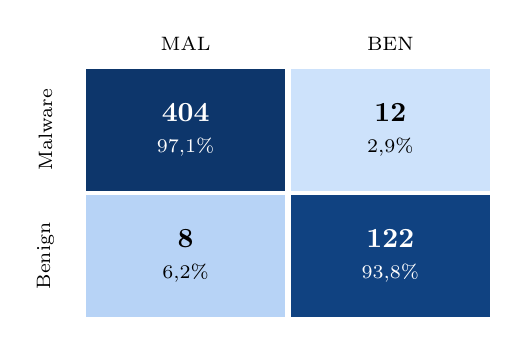
\begin{tikzpicture}[x=2.6cm,y=1.6cm,font=\normalsize]
\definecolor{cm900}{RGB}{13,54,107}
\fill[cm900] (0,0) rectangle ++(0.97,-0.97);
\node[text=white,align=center] at (0.485,-0.485) {\textbf{404}\\[-1pt]{\scriptsize 97,1\%}};
\definecolor{cm901}{RGB}{205,226,251}
\fill[cm901] (1,0) rectangle ++(0.97,-0.97);
\node[text=black,align=center] at (1.485,-0.485) {\textbf{12}\\[-1pt]{\scriptsize 2,9\%}};
\definecolor{cm910}{RGB}{183,211,246}
\fill[cm910] (0,-1) rectangle ++(0.97,-0.97);
\node[text=black,align=center] at (0.485,-1.485) {\textbf{8}\\[-1pt]{\scriptsize 6,2\%}};
\definecolor{cm911}{RGB}{16,66,129}
\fill[cm911] (1,-1) rectangle ++(0.97,-0.97);
\node[text=white,align=center] at (1.485,-1.485) {\textbf{122}\\[-1pt]{\scriptsize 93,8\%}};
\node[font=\scriptsize] at (0.485,0.2) {MAL};
\node[font=\scriptsize] at (1.485,0.2) {BEN};
\node[font=\scriptsize,rotate=90] at (-0.2,-0.485) {Malware};
\node[font=\scriptsize,rotate=90] at (-0.2,-1.485) {Benign};
\end{tikzpicture}
\caption{Confusion matrix του πλήρους συστήματος στο στάδιο του LLM. Γραμμές: πραγματική κλάση· στήλες: απόφαση του συστήματος (MAL = \texttt{MALICIOUS}, BEN = \texttt{BENIGN})· σε κάθε κελί το πλήθος πακέτων και το ποσοστό ανά πραγματική κλάση, με την ένταση του χρώματος ανάλογη του ποσοστού.}
\label{fig:confusion_sum}
\end{figure}
